\chapter{Nonlinear \cobra{}}
\label{chap:nln_solver}
The original \cobra{} software utilized the single timestep of the traditional semi-implicit method.
In order to investigate the effects of nonlinear convergence upon the determination of the temporal convergence for a given solution, \cobra{} was modified to enable an iterative global Newton's method.
Then, for effective use of the nonlinear solver, a operator-based scaling method was developed to provide a physically meaningful measure of convergence.
A metric was then developed and tested to aid in the identification of solutions that may not be temporally converged.
This chapter will discuss each of these phases of development as well several implementation specific practicalities that were identified and resolved.

%-------------------------------------------------------------------------------
%-------------------------------------------------------------------------------
%-------------------------------------------------------------------------------
\section{Linear \cobra{}}
\label{sect:linCobraAlg}

\cobra{} utilizes the semi-implicit method as outlined in \sect{subsect:semi_implicit}.
A detailed description of the solution algorithm as implemented will be presented in the following section.
The linearized semi-implicit method is not traditionally cast as a system of nonlinear equations.
The governing equations in the traditional semi-implicit method are not viewed through the lens of a single Newton step for a system of nonlinear equations.
Instead, the view that the linearization is from $\vec{x}^{n}$ to $\vec{x}^{n+1}$, as opposed to $\vec{x}^{n+1, k}$ to $\vec{x}^{n+1, k+1}$, is standard in the literature of linearized system analysis software.
For that reason, the following discussion will present the algorithm from the point of view of a single-shot linearization.

Assuming that all data has been initialized properly, the first step in \cobra{} is a loop over all momentum equations in the domain.
The nonlinear momentum equations, neglecting spatial discretization notation and external sources, are given in \eqref{eqn:nlnLiqMomentumEquation} -- \eqref{eqn:nlnEntMomentumEquation}.

\begin{IEEEeqnarray}{rCl}
\label{eqn:nlnLiqMomentumEquation}
\dot{m}_{l}^{n+1} - \dot{m}_{l}^{n} & = & \frac{\dt{}}{\dx{}}\left(- \sum^{N_{c}}_{i\,=\,1} \left( \don{\alpha_l \rho_l u_l}_{\text{d}} \ave{u}_{\text{a,l}} \cdot \vec{\bar{A}}\right)_{i}^{n}
 - \ave{\alpha_{l}}_{\text{a}}^{n} \nabla P^{\,n+1} + g \ave{\alpha_l \rho_l}_{\text{a}}^{n} - K^{n}_{wl}(\dot{m}_l^{n+1})^2 \right. \nonumber \\
 & + & \left. K^{n}_{i,gl}(\dot{m}^{n+1}_l - \dot{m}_g^{n+1})^2 - \left[(1 - \eta)\Gamma u^{'} + S u^{'}\right]^{n}\vphantom{\sum_{N_{k}}}\right) \\
\label{eqn:nlnGasMomentumEquation}
\dot{m}_{g}^{n+1} - \dot{m}_{g}^{n} & = & \frac{\dt{}}{\dx{}}\left(- \sum^{N_{c}}_{i\,=\,1} \left( \don{\alpha_g \rho_g u_g}_{\text{d}} \ave{u}_{\text{a},g}  \cdot \vec{\bar{A}}\right)_{i}^{n} - \ave{\alpha_{g}}_{\text{a}}^{n} \nabla P^{\,n + 1} + g \ave{\alpha_g \rho_g}_{\text{a}}^{n} - K^{n}_{wg}(\dot{m}_g^{n+1})^2 \right.\nonumber \\
& - & \left. K^{n}_{i,gl}(\dot{m}^{n+1}_l - \dot{m}_g^{n+1})^2 -K^{n}_{i,ge}(\dot{m}^{n+1}_e - \dot{m}_g^{n+1})^2 + \left[\Gamma u^{'}\right]^{n}\vphantom{\sum_{N_{k}}}\right) \\
\label{eqn:nlnEntMomentumEquation}
\dot{m}_{e}^{n+1} - \dot{m}_{e}^{n} & = & \frac{\dt{}}{\dx{}}\left(- \sum^{N_{c}}_{i\,=\,1} \left( \don{\alpha_e \rho_l u_e}_{\text{d}} \ave{u}_{\text{a},e}  \cdot \vec{\bar{A}}\right)_{i}^n -\ave{\alpha_{e}}_{\text{a}}^{n} \nabla P^{\,n+1} + g \ave{\alpha_e \rho_l}_{\text{a}}^{n} - K^{n}_{we}(\dot{m}_e^{n+1})^2\right. \nonumber \\
&+& \left. K^{n}_{i,ge}(\dot{m}^{n+1}_e - \dot{m}_g^{n+1})^2 - \left[ \eta \Gamma u^{'} - S u^{'}\right]^{n}\vphantom{\sum_{N_{k}}}\right)
\end{IEEEeqnarray}

In the above equations the flux terms are summed over $N_{c}$, which indicates the number of continuity volumes to which a given momentum volume connects.
The coefficients $K$ represent effective wall and interfacial friction factors calculated using parameters only from time $n$.
The transfer of momentum associated with the interfacial transfer of mass is also explicitly evaluated.
The vector notation for the three momenta, \momVec{}, is defined by \eqref{eqn:momentumVector}.

\begin{equation}
\label{eqn:momentumVector}
\momVec{} = \begin{bmatrix}
\dot{m}_{l} \\
\dot{m}_{g} \\
\dot{m}_{e}
\end{bmatrix}
\end{equation}

The terms in the momentum equations that are evaluated at their new-time values are then linearized about their old-time values.
This includes the momenta, $\momVec{}^{n}$, and the pressure, $P^{n}$, giving \eqref{eqn:linLiqMomentumEquation} - \eqref{eqn:linEntMomentumEquation}.

\begin{IEEEeqnarray}{rCl}
\label{eqn:linLiqMomentumEquation}
\dot{m}_{l}^{n+1} - \dot{m}_{l}^{n} & = & \frac{\dt{}}{\dx{}}\left(- \sum^{N_{c}}_{i\,=\,1} \left( \don{\alpha_l \rho_l u_l}_{\text{d}} \ave{u}_{\text{a},l} \cdot \vec{\bar{A}}\right)_{i}^{n}
 -\ave{\alpha_{l}}_{\text{a}}^{n} \nabla P^{\,n} -\ave{\alpha_{l}}_{\text{a}}^{n} \delta (\nabla P) + g \ave{\alpha_l \rho_l}_{\text{a}}^{n} \right. \nonumber \\
  & + & K^{n}_{wl}(\dot{m}_l^{n})^{2} - 2 K^{n}_{wl}\dot{m}_l^{n}\dot{m}_l^{n+1} - K^{n}_{i,gl}(\dot{m}^{n}_l - \dot{m}_g^{n})^2  \nonumber \\
 & + & \left. 2 K^{n}_{i,gl}(\dot{m}^{n}_l - \dot{m}_g^{n})(\dot{m}^{n+1}_l - \dot{m}_g^{n+1}) - \left[(1 - \eta)\Gamma u^{'} + S u^{'}\right]^{n}\vphantom{\sum_{N_{k}}}\right) \\
\label{eqn:linGasMomentumEquation}
\dot{m}_{g}^{n+1} - \dot{m}_{g}^{n} & = & \frac{\dt{}}{\dx{}}\left(- \sum^{N_{c}}_{i\,=\,1} \left( \don{\alpha_g \rho_g u_g}_{\text{d}} \ave{u}_{\text{a},g} \cdot \vec{\bar{A}}\right)_{i}^{n}
 -\ave{\alpha_{g}}_{\text{a}}^{n} \nabla P^{\,n} -\ave{\alpha_{g}}_{\text{a}}^{n} \delta (\nabla P) + g \ave{\alpha_g \rho_g}_{\text{a}}^{n}  \right. \nonumber \\
  & + & K^{n}_{wg}(\dot{m}_g^{n})^{2} + K^{n}_{i,gl}(\dot{m}^{n}_l - \dot{m}_g^{n})^2 + K^{n}_{i,ge}(\dot{m}^{n}_e - \dot{m}_g^{n})^2 + \left[\Gamma u^{'}\right]^{n} \nonumber \\
 & - & 2 K^{n}_{i,gl}(\dot{m}^{n}_l - \dot{m}_g^{n})(\dot{m}^{n+1}_l - \dot{m}_g^{n+1}) - 2 K^{n}_{wg}\dot{m}_g^{n}\dot{m}_g^{n+1} \nonumber \\
 & - & \left. 2 K^{n}_{i,ge}(\dot{m}^{n}_e - \dot{m}_g^{n})(\dot{m}^{n+1}_e - \dot{m}_g^{n+1})\vphantom{\sum_{N_{k}}}\right) \\
\label{eqn:linEntMomentumEquation}
\dot{m}_{e}^{n+1} - \dot{m}_{e}^{n} & = & \frac{\dt{}}{\dx{}}\left(- \sum^{N_{c}}_{i\,=\,1} \left( \don{\alpha_e \rho_e u_e}_{\text{d}} \ave{u}_{\text{a},e} \cdot \vec{\bar{A}}\right)_{i}^{n}
 -\ave{\alpha_{e}}_{\text{a}}^{n} \nabla P^{\,n} - \ave{\alpha_{e}}_{\text{a}}^{n} \delta (\nabla P ) + g \ave{\alpha_e \rho_e}_{\text{a}}^{n}  \right. \nonumber \\
  & + & K^{n}_{we}(\dot{m}_e^{n})^{2} - 2 K^{n}_{we}\dot{m}_e^{n}\dot{m}_e^{n+1} - K^{n}_{i,ge}(\dot{m}^{n}_e - \dot{m}_g^{n})^2  \nonumber \\
 & + & \left. 2 K^{n}_{i,ge}(\dot{m}^{n}_e - \dot{m}_g^{n})(\dot{m}^{n+1}_e - \dot{m}_g^{n+1}) -\left[ \eta \Gamma u^{'} - S u^{'}\right]^{n}\vphantom{\sum_{N_{k}}}\right)
\end{IEEEeqnarray}

The momentum equations, \eqref{eqn:linLiqMomentumEquation} - \eqref{eqn:linEntMomentumEquation}, are now linear in the unknown variables $\momVec{}^{n+1}$.
These equations are then solved for the unknown new time momenta, $\momVec{}^{n+1}$.
The $\delta P$ is left as an unknown, creating an additional unknown on the right-hand side of the linear system.
The resulting system is of the form $\displaystyle \vec{A}_{j} \momVec{}_{j}^{n+1} = \vec{a}_{j} + \sum^{N_{c}}_{i\,=\,1} \vec{b}_{j} \delta P_{i}$.
The solution of this linear system is expressed in \eqref{eqn:momStar}.

\begin{equation}
\label{eqn:momStar}
\momVec{}_{j}^{n+1} = \momVec{}^{*}_{j} + \sum^{N_{c}}_{i\,=\,1} \frac{\partial \momVec{}_{j}}{\partial P_{i}} \delta P_{i}
\end{equation}

The definition for the new-time momenta is a function of the as of yet unknown changes in pressures that occur in the continuity volumes connected by the momentum volume.
The $\momVec{}^{*}$ vector on the right-hand side of \eqref{eqn:momStar} contains the tentative new time momenta.
Once all of the momentum equations have been solved in the above manner, providing estimated new-time momenta for each momentum volume, the domain's continuity volumes are then looped over.
The continuity equations used in this work, omitting external sources, are shown in \eqref{eqn:nlnNcgMassEquation} -- \eqref{eqn:nlnLiqMassEquation}. 
The new-time velocities used for advection in the continuity equations are defined with the new-time momenta, \eqref{eqn:momStar}, in conjunction with \eqref{eqn:si_vel}.

\begin{IEEEeqnarray}{rCl}
\label{eqn:nlnNcgMassEquation}
V_c \left[(\alpha_g \rho_{n})^{n+1}\right. & - & \left. (\alpha_g \rho_{n})^{n}\right] = -\dt{} \sum^{N_{f}}_{i\,=\,1}\left( \don{\alpha^{n}_g \rho^{n}_{n}}^{n+1}_{d} u^{n+1}_g  \cdot \vec{\bar{A}}\right)_{i} \\
\label{eqn:nlnVapMassEquation}
V_c\left[ \left(\alpha_g \rho_v \right)^{n+1}\right. &-& \left. \left(\alpha_g \rho_v \right)^{n}\right] = - \dt{} \sum^{N_{f}}_{i\,=\,1} \left( \don{\alpha^{n}_g \rho^{n}_v}^{n+1}_{d} u^{n+1}_g  \cdot \vec{\bar{A}}\right)_{i} + 
\dt{} \Gamma^{n+1} \\
\label{eqn:nlnGasEnergyEquation}
V_c \left[ \left( \alpha_g \rho_g h_g \right)^{n+1} \right. & - & \left. \left( \alpha_g \rho_g h_g \right)^{n} - \alpha^{n}_g ( P^{\,n+1} - P^{n} )\right ] = \dt{} \left[q_{wg} + \Gamma h^{'}_v + q_{i,v} + q_{gl}\right]^{n+1} \nonumber \\
&- &\dt{} \sum^{N_{f}}_{i\,=\,1} \left(  \don{\alpha^{n}_g \rho^{n}_g h^{n}_{g}}^{n+1}_{d} u^{n+1}_g  \cdot \vec{\bar{A}}\right)_{i} \\
\label{eqn:nlnLiqEnergyEquation}
V_c\left[\left( \alpha_l \rho_l h_l \right)^{n+1} \right. & - & \left. \left( \alpha_l \rho_l h_l \right)^{n} - \alpha^{n}_l (P^{\,n+1} - P^{\,n}) \right] = \dt{} \left[q_{wl} -\Gamma h^{'}_l +  q_{i,l} - q_{gl}\right]^{n+1} \nonumber \\
& -& \dt{} \sum^{N_{f}}_{i\,=\,1} \left( \don{\alpha^{n}_l \rho^{n}_l h^{n}_l}^{n+1}_{d} u^{n+1}_l \cdot \vec{\bar{A}} + \don{\alpha^{n}_e \rho^{n}_l h^{n}_l}^{n+1}_{d} u^{n+1}_e  \cdot \vec{\bar{A}}\right)_{i} \\
\label{eqn:nlnEntMassEquation}
V_c \left[ \left(\alpha_e \rho_l \right)^{n+1}\right. & - & \left. \left(\alpha_e \rho_l \right)^{n} \right]= -\dt{} \sum^{N_{f}}_{i\,=\,1}\left( \don{\alpha^{n}_e \rho^{n}_l}^{n+1}_{d} u^{n+1}_e  \cdot \vec{\bar{A}}\right)_{i}+ \dt{}\left[ S -\eta\Gamma \right]^{n+1} \\
\label{eqn:nlnLiqMassEquation}
V_c \left[ \left(\alpha_l \rho_l \right)^{n+1} \right. & - & \left. \left(\alpha_l \rho_l \right)^{n} \right]=  -\dt{} \sum^{N_{f}}_{i\,=\,1}\left( \don{\alpha^n_l \rho^n_l}^{n+1}_{d} u^{n+1}_l  \cdot \vec{\bar{A}}\right)_{i} \nonumber \\
&- &\dt{}\left[(1-\eta)\Gamma + S \right]^{n+1}
\end{IEEEeqnarray}

Unlike the momentum equations, the continuity equations are linearized with variables other than their conserved quantities, \eqref{eqn:independentVariables}.
This creates a more complicated linearization than that used for the momentum equations.
The new-time variables in \eqref{eqn:nlnNcgMassEquation} -- \eqref{eqn:nlnLiqMassEquation} are linearized about the old-time variables with respect to the continuity variables in \eqref{eqn:independentVariables}.
The use of \eqref{eqn:momStar} in defining the new-time velocities introduces inter-continuity volume coupling through the momentum equations' dependency upon changes in pressure, $\delta P$.

\begin{equation}
\label{eqn:linSystem}
\underbrace{\left[\vec{Z}_{c, j}\right]}_{6\, \text{x}\, 6 + N_{f}} \delta \vec{C}_{j} = \vec{r}_{c,j}
\end{equation}

With the addition of the unknown pressure updates via the momenta, the six linearized continuity equations now form the linear system \eqref{eqn:linSystem}.
Additionally, while the momentum equations were fully expanded to solve for the new-time conserved quantities directly, the continuity equations instead solve for their associated updates, \eqref{eqn:linearUpdate}.

\begin{equation}
\label{eqn:linearUpdate}
\delta \vec{C}_{j} \equiv 
\begin{bmatrix}
\delta ( \alpha_{g} P_{n} )_j \\
\delta \alpha_{g, j} \\
\delta ( \alpha_{g} h_v )_j \\
\delta ( (1 - \alpha_{g} ) h_l )_j \\
\delta \alpha_{e,j} \\
\delta P_j \\ 
\delta P_i \\
\vdots \\
\delta P_{N_{f}}
\end{bmatrix}
=
\begin{bmatrix}
( \alpha_{g} P_{n})_{j}^{n+1} - (\alpha_{g} P_{g} )_{j}^{n} \\
\alpha^{n+1}_{g,j} - \alpha^{n}_{g,j} \\
( \alpha_{g} h_{v} )_{j}^{n+1} - ( \alpha_{g} h_{v} )_{j}^{n} \\
( ( 1 - \alpha_{g} ) h_{l} )_{j}^{n+1} - ( ( 1 - \alpha_{g} ) h_{l} )_{j}^{n} \\
\alpha^{n+1}_{e,j} - \alpha^{n}_{e,j} \\
 P_{j}^{n+1} - P_{j}^{n} \\
 P_{i}^{n+1} - P_{i}^{n} \\
 \vdots \\
 P_{N_{f}}^{n+1} - P_{N_{f}}^{n}
\end{bmatrix}
\end{equation}

Each continuity volume's linearized system of equations, \eqref{eqn:linSystem}, is subjected to partial LU decomposition without pivoting.
The lower triangular matrix has a unit diagonal.
The sixth equation in the upper-triangular system is then scaled by its diagonal.
This upper-triangular rectangular system for each continuity volume is then stored for later back-substitution.
Since the pressure update corresponds to the last row in the system of equations, this allows for the isolation of the pressure updates.
The last row of each continuity volume's \eqref{eqn:linSystem} is then formed into a global pressure matrix, $\vec{A}_{N,N}$, and its associated right-hand side, $\vec{r}$.

The two loops, one over the momentum volumes and one over the continuity volumes, form a single group of operations that act upon a given domain.
This grouping will be known hereafter as assembling the pressure matrix for a given domain.
\alg{alg:xschem} shows the two loops and their associated actions.

\begin{algo}[ht!]
\setlength{\baselineskip}{0.625\baselineskip}
\begin{algorithmic}[1]
\Loop \; Momentum Volumes
	\Calculate $\vec{J}_{m, j}$, $\vec{a}_{j}$, and $\vec{b}_{j}$
	\Calculate $\momVec{}^{*}$ and $\frac{\partial \momVec{}}{\partial P}$
	\Calculate $\vec{F}_{m, j}$	
	\Calculate $\vec{S}_{m, j}$	
\EndLoop
\Loop \; Continuity Volumes
   	\Calculate $\vec{Z}_{c,j}$ and $\vec{r}_{c, j}$
 	\Calculate $\vec{F}_{c, j}$	
	\Calculate $\vec{S}_{c, j}$	
   	\Calculate $\vec{U}_{c, j} = \vec{L}_{c, j}^{-1} \vec{Z}_{c, j}$
   	\Calculate $\vec{r}^{*}_{c, j} = \vec{L}_{c, j}^{-1} \vec{r}_{c, j}$
   	\Set Scale $\vec{U}[6, :]_{c, j}$ and $\vec{r}[6]^{*}_{c, j}$ by $\vec{U}[6,6]_{c, j}$
   	\Set $\vec{A}_{i, :} = \vec{U}[6,:]_{c, j}$
   	\Set $\vec{res}_{i} = \vec{r}[6]^{*}_{c, j}$
\EndLoop
\end{algorithmic}
\caption{Assembling Pressure Matrix}
\label{alg:xschem}
\end{algo}

\begin{equation}
\label{eqn:pressureUpdateSystem}
\vec{A} \vec{\delta P} = \vec{res}
\end{equation}

The system, \eqref{eqn:pressureUpdateSystem}, is then solved to determine the pressure updates for the whole domain.
A loop over each continuity volume is then performed so that the pressure update can be used in solving its associated upper triangular system for the updates to the other five continuity variables in \eqref{eqn:linearUpdate}.
As the loop over the continuity volume is progressing, any momentum volume connected to the given continuity volume will have its momenta updated according to \eqref{eqn:momStar} to include the contribution from that continuity volumes' change in pressure. 
This update loop is shown in \alg{alg:updateVariables}.

\begin{algo}[ht!]
\setlength{\baselineskip}{0.625\baselineskip}
\begin{algorithmic}[1]
\Loop \; Continuity Volumes
	\Solve $\vec{U}_{c, j} \delta \vec{C}_{c, j} = \vec{r}^{*}_{c, j}$ using $\vec{\delta P}$		
	\Loop \; Connected Flow Paths
		\Set $\momVec{}^{*}_{j} \pluseq sig \cdot \frac{\partial \momVec{}}{\partial P} \delta P_{j}$
	\EndLoop
\EndLoop
\end{algorithmic}
\caption{Updating Continuity and Momentum Variables}
\label{alg:updateVariables}
\end{algo}

Upon completion of this process, a single timestep is considered to have been taken.
The complete linear process is outlined in \alg{alg:linCobraAlgorithm}.

\begin{algo}[ht!]
\setlength{\baselineskip}{0.625\baselineskip}
\begin{algorithmic}[1]
\Require $\vec{x}^{0}$ and $t^{0}$
\Set $n = 0$
\Loop \; Transient Loop
    \Set $t^{n+1} : = t^{n} + \dt{}$
	\Algorithm Assemble Linear Pressure Matrix \Comment{\alg{alg:xschem}}
   	\Solve $\vec{A} \vec{\delta P} = \vec{res}$
	\Algorithm Update Linear Variables \Comment{\alg{alg:updateVariables}}
	\Set $n = n + 1$
\EndLoop
\end{algorithmic}
\caption{Linear \cobra{} algorithm.}
\label{alg:linCobraAlgorithm}
\end{algo}

The solution obtained via this process is subjected to several physical and computational limits discussed in \sect{sect:miscConcerns}.

%-------------------------------------------------------------------------------
%-------------------------------------------------------------------------------
%-------------------------------------------------------------------------------
\section{Nonlinear \cobra{}}
\label{sect:nlnCobraSolver}
As obtained, the \cobra{} software used the timestep of the semi-implicit method as outlined in \sect{sect:linCobraAlg}.
In order to evaluate the subdomain nonlinear refinement algorithm, \cobra{} needed to be modified to be able to take multiple Newton steps within a given timestep.
To achieve this goal, several objectives were met.
First, the software routines that calculated portions of $\vec{F}(\vec{x}^{k})$ and $\vec{J}(\vec{x}^{k})$ were evaluated and transitioned to the proper nonlinear discretization.
Second, a method to identify the active portion of the domain was developed to correctly construct $\vec{x}^{k}$ and $\vec{F}^{k}$.
Lastly, a Newton loop algorithm was implemented.
This section will describe work done to meet the above objectives.

%-------------------------------------------------------------------------------
%-------------------------------------------------------------------------------
%-------------------------------------------------------------------------------
\subsection{Evaluation of Discretization}
\label{subsect:nonlinearDiscretization}

Given the formation of the governing equations from \sect{sect:linCobraAlg}, several modifications were required to implement the nonlinear solver.
Using an iterative nonlinear solver requires that the governing equations be linearized about a tentative new-time value $\vec{x}^{n+1, k}$; this differs from the linear case in which the linearization occurs about the old-time values $\vec{x}^{n}$.
First, the correct linearization about a new-time guess value as opposed to the old-time value needed to be implemented.
Each Newton step is an incremental change in the new-time variable, not a change in the independent parameters over a timestep.
Second, memory saving techniques had been employed in the construction of the linear solver that precluded more than one Newton step.
In particular, there had been the implicit assumption within the software that the first Newton iterate, $\vec{x}^{n+1, 0}$, was the old-time variable $\vec{x}^{n}$.
This design decision required that all subroutines involved with the evaluation of the components of both the nonlinear residual and its Jacobian be vetted for accurate usage of variables.
Third, the assumption that $\vec{x}^{n+1, k} = \vec{x}^{n}$ produced source code that was inconsistent with an iterative Newton method.
The source code was modified to reflect the intended discretization of the governing conservation laws.
To do this, areas had to be identified where: there were implicit cancellation of terms, the new-time variables were used in place of old-time variables, and the old-time variables were used in place of new-time variables.
This required each of the Fortran procedures involved with the calculation of the various physical parameters and operators to be evaluated to determine if the variables being used were correct.
Where appropriate, the software was changed to reflect the distinction between old-time and tentative new-time variables and to introduce terms that had been assumed to be equal to zero.
Additionally, upon verification of the proper discretization of the governing equations, several architectural changes were also made to expedite the implementation of the nonlinear solver.

%-------------------------------------------------------------------------------
%-------------------------------------------------------------------------------
%-------------------------------------------------------------------------------
\subsection{Active Domain Determination}
\label{subsect:activeDomainDetermination}
In \cobra{} the smallest geometric component that can be input is the channel.
As mentioned in \sect{sect:geometry} channels inherit their geometric properties from the section in which they reside.
To create geometrically complicated problems, it is possible to enforce zero momentum in a given momentum volume, decoupling adjacent continuity volumes by eliminating the flow paths that connect them.
This constraint is known as a no-flow boundary condition, and it allows more complicated models to be created by isolating portions of the domain.
If an isolated domain is not connected to an external boundary condition, then it is marked as an inactive region.
The inactive regions are thermodynamically isolated and form a closed system.
These areas of the domain do not impact the solution in the portion of the domain that has boundary values, known as the active region.
After evaluating several prototypical models, it was determined that a large portion of the domain of these problems were thermodynamically isolable.
\fig{fig:activeDomain} shows an example of a domain with inactive regions.
The inactive portions of the domain are marked with grey, the active with white, and the external boundary conditions with black.
Inter-channel flow paths are marked with dashed lines.

\begin{figure}[ht!]
\centering
\tikzsetnextfilename{images/active_inactive_eps}
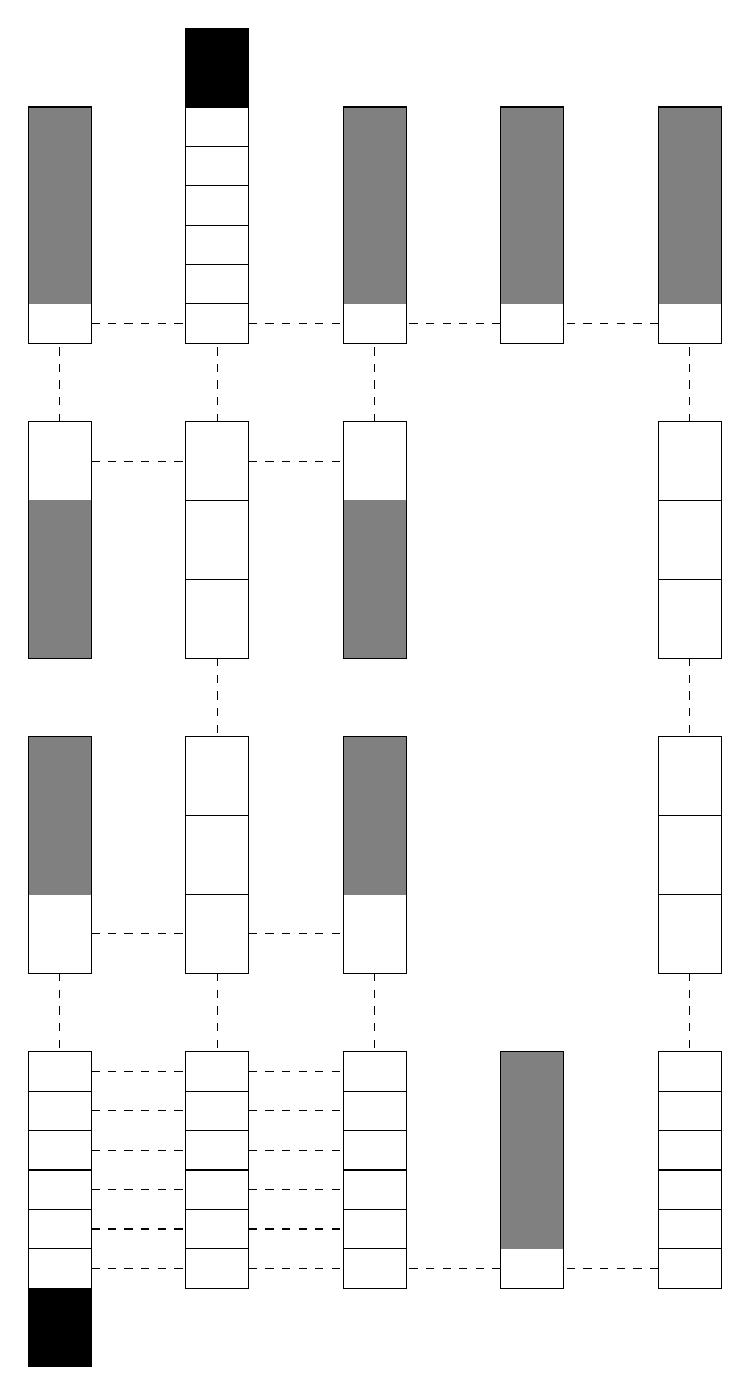
\begin{tikzpicture}
% \draw [thick] (-2,-3) rectangle (2,3);
% \draw [<->] (3.5,-3) -- (3.5,3);
% \draw (3.25,-3) -- (3.75,-3);
% \draw (3.25,3) -- (3.75,3);
% \draw [<->] (-2,-3.75) -- (2,-3.75);
% \draw (-2,-3.5) -- (-2,-4);
% \draw (2,-3.5) -- (2,-4);

% Middle rows of gray
\filldraw [gray] (-4.4,.5) rectangle (-3.6,2.5);
\filldraw [gray] (-.4,.5) rectangle (.4,2.5);
\filldraw [gray] (-4.4,-.5) rectangle (-3.6,-2.5);
\filldraw [gray] (-.4,-.5) rectangle (.4,-2.5);

% Top row of gray
\filldraw [gray] (-4.4,7.5) rectangle (-3.6,5);
\filldraw [gray] (-.4,7.5) rectangle (.4,5);
\filldraw [gray] (1.6,7.5) rectangle (2.4,5);
\filldraw [gray] (3.6,7.5) rectangle (4.4,5);

% Bottom row of gray
\filldraw [gray] (1.6,-7) rectangle (2.4,-4.5);

% Top and bottom row of rectangles
\foreach \x in {-4,-2,...,4}
\foreach \y in {-6,6}
{
\draw (\x,\y) +(-.4,-1.5) rectangle ++(.4,1.5);
}

% Middle rows of rectangles
\foreach \x in {-4,-2,0,4}
\foreach \y in {-2,2}
{
\draw (\x,\y) +(-.4,-1.5) rectangle ++(.4,1.5);
}

%Horizontal partitions
\foreach \y in {-7.5,-7,...,-4.5,-2.5,-1.5,1.5,2.5,4.5,5,...,7.5}
\draw (-1.6,\y) -- (-2.4,\y);

\foreach \y in {-7.5,-7,...,-4.5,-2.5,-1.5,1.5,2.5}
\draw (3.6,\y) -- (4.4,\y);

\foreach \y in {-7.5,-7,...,-4.5}
\draw (-3.6,\y) -- (-4.4,\y);

\foreach \y in {-7.5,-7,...,-4.5}
\draw (-.4,\y) -- (.4,\y);

% Vertical connections
\foreach \x in {-4,-2,0,4}
\draw [dashed] (\x,3.5) -- (\x,4.5);

\foreach \x in {-2,4}
\draw [dashed] (\x,.5) -- (\x,-.5);

\foreach \x in {-4,-2,0,4}
\draw [dashed] (\x,-3.5) -- (\x,-4.5);

% Black rectangles
\filldraw [black] (-1.6,7.5) rectangle (-2.4,8.5);

\filldraw [black] (-3.6,-7.5) rectangle (-4.4,-8.5);

%Horizontal connentions
\foreach \y in {4.75,3,-3,-4.75,-5.25,...,-7.25}
\draw [dashed] (-3.6,\y) -- (-2.4,\y);

\foreach \y in {4.75,3,-3,-4.75,-5.25,...,-7.25}
\draw [dashed] (-1.6,\y) -- (-.4,\y);

\foreach \y in {4.75,-7.25}
\draw [dashed] (1.6,\y) -- (.4,\y);

\foreach \y in {4.75,-7.25}
\draw [dashed] (3.6,\y) -- (2.4,\y);

\end{tikzpicture}
\caption{A Domain with Inactive Regions}
\label{fig:activeDomain}
\end{figure}

Originally, \cobra{} would solve the momentum and continuity equations at every defined location in the problem.
The pressure matrix, $\vec{A}_{N\,x\,N}$, was sized based upon the number of volumes in the domain, $N$, not the number of active volumes, $N_{a}$.
During development it was determined that those continuity and momentum volumes which were in the inactive region would be pruned from the the simulation.
While the additional costs of including these volumes in the simulation have historically been acceptable, the use of an iterative solver would amplify the computational time spent in those regions to an unacceptable degree.
Removing these inactive volumes saved computational time by precluding the evaluation of the residuals at those locations and by modifying the size of the pressure system \eqref{eqn:pressureUpdateSystem}.
Additionally, since the inactive regions of the problem are interpreted as not being part of the system being modeled, including their equations in the residual would not provide an accurate measure of convergence.

To determine which areas of the domain were active and which ones were inactive, a geometry traversing routine was written.
This routine parses the \cobra{} input file and creates an adjacency list data structure to represent the active portion of the domain.
The data structure allowed the active volumes to be treated independently from the memory structure of the software.
Once the active volumes were identified, the way in which the domain information was stored in memory was changed.

%-------------------------------------------------------------------------------
%-------------------------------------------------------------------------------
%-------------------------------------------------------------------------------
\subsection{Nonlinear Algorithm}
\label{subsect:nlnCobraAlgo}

During this research, the \cobra{} software was transitioned from the linear solver outlined in \sect{sect:linCobraAlg} to a nonlinearly-convergent solver. 
The solution method selected for the nonlinear system was the iterative Newton's method.
Newton's method uses successive linearizations to find a solution vector that adequately satisfies the system of discrete nonlinear equations.
The algorithmic outline for the nonlinear solver is presented in \alg{alg:nlnCobraAlgorithm}.

\begin{algo}[ht!]
\setlength{\baselineskip}{0.625\baselineskip}
\begin{algorithmic}[1]
\Require $\vec{x}^{0}$ and $t^{0}$
\Set $n = 0$
\Loop \; Transient Loop
    \Set $t^{n+1} : = t^{n} + \dt{}$
    \Set $k = 0$
	\Algorithm Assemble Nonlinear Pressure Matrix	 \Comment{\alg{alg:xschem}}
	\Solve $\vec{A}^{k} \vec{\delta P}^{k} = \vec{res}^{k}$
	\Algorithm Update Nonlinear Variables \Comment{\alg{alg:updateVariables}} 
    \Loop \; Newton Loop
		\Algorithm Assemble Nonlinear Pressure Matrix \Comment{\alg{alg:xschem}}
		\Algorithm Convergence Determination \Comment{\alg{alg:nlnConvergence}}
		\If{ \textbf{end} Newton loop}
			\State \textbf{break} Newton Loop 
		\EndIf		
		\Set $k \pluseq 1$
		\Solve $\vec{A}^{k} \vec{\delta P}^{k} = \vec{res}^{k}$
		\Algorithm Update Nonlinear Variables \Comment{\alg{alg:updateVariables}}
	\EndLoop
	\Set $n \pluseq 1$
\EndLoop
\end{algorithmic}
\caption{Nonlinear \cobra{} algorithm.}
\label{alg:nlnCobraAlgorithm}
\end{algo}

The following section will roughly parallel \alg{alg:nlnCobraAlgorithm}.
First, the method by which the nonlinear residuals are evaluated and calculated is presented.
This portion will be an extension of the procedure discussed in \sect{sect:linCobraAlg} and outlined in \alg{alg:xschem}.
Second, the process through which the Newton vector is updated, \alg{alg:updateVariables}, is expounded upon and  discussed.
Lastly, the method by which determination of convergence is discussed and is presented in \alg{alg:nlnConvergence}.

A detailed discussion of process through which the nonlinear residuals are evaluated and the pressure matrix is assembled will now be presented.
Two quantities that are important to the iterative solver are the residual vector, $\vec{F}^{k}$, and the update vector, $\delta \vec{x}$.
The update vector represents the changes in the solution vector that result from a given Newton step.
The residual vector is composed of the residuals from the governing partial differential equations that are being solved.
Every momentum volume has associated with it three momentum equation residuals \eqref{eqn:nlnLiqMomentumResidual} -- \eqref{eqn:nlnEntMomentumResidual}.

\begin{IEEEeqnarray}{lCl}
\label{eqn:nlnLiqMomentumResidual}
F^{k}_{m, l} & = & \dot{m}_{l}^{n+1, k} - \dot{m}_{l}^{n} + \frac{\dt{}}{\dx{}}\left(\sum^{N_{c}}_{i\,=\,1} \left( \don{\alpha_l \rho_l u_l}_{\text{d}} \ave{u}_{\text{a},l} \cdot \vec{\bar{A}}\right)_{i}^{n}
 +\ave{\alpha_l}^{n}_{\text{a}} \nabla P^{\,n+1, k} - g \ave{\alpha_l \rho_l}_{\text{a}}^{n} \right. \nonumber \\
& + & \left. K^{n}_{wl}(\dot{m}_l^{n+1, k})^2 - K^{n}_{i,gl}(u^{n+1, k}_{l} - u^{n+1,k}_{g})^2 + \left[(1 - \eta)\Gamma u^{'} + S u^{'}\right]^{n} \vphantom{\sum_{N_{k}}}\right) \\
\label{eqn:nlnGasMomentumResidual}
F^{k}_{m, g} & = & \dot{m}_{g}^{n+1,k} - \dot{m}_{g}^{n} + \frac{\dt{}}{\dx{}}\left(\sum^{N_{c}}_{i\,=\,1} \left( \don{\alpha_g \rho_g u_g}_{\text{d}} \ave{u}_{\text{a},g}  \cdot \vec{\bar{A}}\right)_{i}^{n}  +\ave{\alpha_g}^{n}_{\text{a}} \nabla P^{\,n+1, k} - g \ave{\alpha_g \rho_g}_{\text{a}}^{n} \right.\nonumber \\
& + & \left. K^{n}_{wg}(\dot{m}_g^{n+1, k})^2 + K^{n}_{i,gl}(u^{n+1, k}_{l} - u^{n+1, k}_{g})^2 + K^{n}_{i,ge}(u^{n+1,k}_{e} - u^{n+1,k}_{g})^2 - (\Gamma u^{'})^{n} \vphantom{\sum_{N_{k}}}\right) \\
\label{eqn:nlnEntMomentumResidual}
F^{k}_{m, e} & = & \dot{m}_{e}^{n+1, k} - \dot{m}_{e}^{n} + \frac{\dt{}}{\dx{}}\left(\sum^{N_{c}}_{i\,=\,1} \left( \don{\alpha_e \rho_l u_e}_{\text{d}} \ave{u}_{\text{a},e}  \cdot \vec{\bar{A}}\right)_{i}^{n} + \ave{\alpha_{e}}^{n}_{\text{a}} \nabla P^{\,n+1, k} - g \ave{\alpha_e \rho_l}^{n}_{\text{a}} \right. \nonumber \\
& + & \left. K^{n}_{we}(\dot{m}_e^{n+1, k})^2 - K^{n}_{i,ge}(u^{n+1, k}_{e} - u^{n+1, k}_{g})^2 + \left[\eta \Gamma u^{'} - S u^{'}\right]^n\vphantom{\sum_{N_{k}}}\right)
\end{IEEEeqnarray}

The three momentum equations are linearized about their tentative new-time values.
The system of linear equations that results from the linearization is shown in \eqref{eqn:nlnMomentumSystem}.

\begin{equation}
\label{eqn:nlnMomentumSystem}
\frac{\partial\, \vec{F}^{k}_{m}}{\partial \dot{m}^{n+1}_{l}} \delta \dot{m}_{l}^{k} + \frac{\partial\, \vec{F}^{k}_{m}}{\partial \dot{m}^{n+1}_{g}} \delta \dot{m}_{g}^{k} + \frac{\partial\, \vec{F}^{k}_{m}}{\partial \dot{m}^{n+1}_{e}} \delta \dot{m}_{e}^{k} + \sum_{i\,=\,1}^{N_{c}} \frac{\partial\, \vec{F}^{k}_{m}}{\partial P_{i}} \delta P_{i}^{k} = - \vec{F}^{k}_{m}
\end{equation}

The first three columns on the right-hand side of \eqref{eqn:nlnMomentumSystem} represent the derivatives of the momentum residual with respect to the momentum variables.
These three columns will be referred to as the Jacobian matrix for a given momentum volume, $\vec{J}^{k}_{m}$, defined in \eqref{eqn:momentumJacobian}.

\begin{equation}
\label{eqn:momentumJacobian}
\vec{J}^{k}_{m} = 
\begin{bmatrix}
\frac{\partial F^{k}_{m,l}}{\partial \dot{m}^{n+1}_{l}} & \frac{\partial F^{k}_{m,l}}{\partial \dot{m}^{n+1}_{g}} & \frac{\partial F^{k}_{m,l}}{\partial \dot{m}^{n+1}_{e}} \\
\frac{\partial F^{k}_{m,g}}{\partial \dot{m}^{n+1}_{l}} & \frac{\partial F^{k}_{m,g}}{\partial \dot{m}^{n+1}_{g}} & \frac{\partial F^{k}_{m,g}}{\partial \dot{m}^{n+1}_{e}} \\
\frac{\partial F^{k}_{m,e}}{\partial \dot{m}^{n+1}_{l}} & \frac{\partial F^{k}_{m,e}}{\partial \dot{m}^{n+1}_{g}} & \frac{\partial F^{k}_{m,e}}{\partial \dot{m}^{n+1}_{e}} \\
\end{bmatrix}
\end{equation}

Using \eqref{eqn:momentumVector} and \eqref{eqn:momentumJacobian}, \eqref{eqn:nlnMomentumSystem} can be expressed as \eqref{eqn:momentumMatrixSystem}.

\begin{equation}
\label{eqn:momentumMatrixSystem}
\vec{J}^{k}_{m} \delta \momVec{}^{k}  = - \vec{F}^{k}_{m} - \sum_{i\,=\,1}^{N_{c}} \frac{\partial\, \vec{F}^{k}_{m}}{\partial P_{i}} \delta P_{i}^{k}
\end{equation}

This system of equations, \eqref{eqn:momentumMatrixSystem}, is then solved for the updated new-time momentum vector via the procedure shown in \eqref{eqn:momentumSolution}.

\begin{IEEEeqnarray}{rcl}
\label{eqn:momentumSolution}
\vec{J}^{k}_{m} \delta \momVec{}^{k} & = & -\vec{F}_{m}^{k} - \sum^{N_{c}}_{i\,=\,1} \frac{\partial \vec{F}^{k}_{m}}{\partial P_{i}} \delta P^{k}_{i} \nonumber \\
\vec{J}^{k}_{m} \left[\momVec{}^{n+1, k + 1} - \momVec{}^{n+1, k} \right] & = & -\vec{F}^{k}_{m} - \sum^{N_{c}}_{i\,=\,1} \frac{\partial \vec{F}^{k}_{m}}{\partial P_{i}} \delta P^{k}_{i} \nonumber \\
\vec{J}^{k}_{m} \momVec{}^{n+1, k + 1} & = & - \vec{F}^{k}_{m} + \vec{J}^{k}_{m} \momVec{}^{n+1, k} - \sum^{N_{c}}_{i\,=\,1} \frac{\partial \vec{F}^{k}_{m}}{\partial P_{i}} \delta P^{k}_{i} \nonumber \\
\momVec{}^{n+1, k + 1} & = & \left[\vec{J}_{m}^{k}\right]^{-1} \left[- \vec{F}^{k}_{m}  + \vec{J}^{k}_{m} \momVec{}^{n+1, k} \right] - \sum^{N_{c}}_{i\,=\,1} \left[\vec{J}^{k}_{m}\right]^{-1} \left[\frac{\partial \vec{F}^{k}_{m}}{\partial P_{i}}\right] \delta P^{k}_{i} \nonumber \\
\momVec{}^{n+1, k + 1} & = & \momVec{}^{n+1, k + \onehalf} + \sum^{N_{c}}_{i\,=\,1} \frac{\partial \momVec{}^{k}}{\partial P_{i}} \delta P^{k}_{i}
\end{IEEEeqnarray}

The variable $\momVec{}^{n+1, k + \onehalf}$, defined in \eqref{eqn:momHalf}, present in \eqref{eqn:momentumSolution} is the iterative analog to $\momVec{}^{*}$ from \eqref{eqn:momStar}.

\begin{IEEEeqnarray}{rcl}
\label{eqn:momHalf}
\momVec{}^{n+1, k + \onehalf} & = & \left[\vec{J}^{k}_{m}\right]^{-1}\left[ \vec{J}^{k}_{m} \momVec{}^{n+1, k}  - \vec{F}^{k}_{m} \right] \nonumber \\
\momVec{}^{n+1, k + \onehalf} & = & \momVec{}^{n+1, k} - \left[\vec{J}^{k}_{m}\right]^{-1}\vec{F}^{k}_{m} \nonumber \\
\momVec{}^{n+1, k + \onehalf} & = & \momVec{}^{n+1, k} + \delta \momVec{}^{*}
\end{IEEEeqnarray}

For algebraic convenience, the update vector, $\delta \momVec{}^{k}$, is defined in \eqref{eqn:momentumUpdate}.

\begin{IEEEeqnarray}{rcl}
\label{eqn:momentumUpdate}
\delta \momVec{}^{k} & = & - \left[\vec{J}_{m}^{k}\right]^{-1} \vec{F}^{k}_{m} - \sum_{i\,=\,1}^{N_{c}} \left[\vec{J}_{m}^{k}\right]^{-1}\left[\frac{\partial\, \vec{F}^{k}_{m}}{\partial P_{i}}\right] \delta P_{i}^{k} \nonumber \\
\delta \momVec{}^{k} & = & \delta \momVec{}^{*} + \sum_{i\,=\,1}^{N_{c}} \frac{\partial \momVec{}}{\partial P_{i}} \delta P_{i}^{k}
\end{IEEEeqnarray}

Likewise, each continuity volume has associated with it six residuals representing the mass and energy equations \eqref{eqn:nlnNcgMassResidual} -- \eqref{eqn:nlnVapMassResidual}.
For a given continuity volume, these six equations are collectively referred to as $\vec{F}_{c}$.

\begin{IEEEeqnarray}{lCl}
\label{eqn:nlnNcgMassResidual}
F^{k}_{c, n} & = & V_c\left[ (\alpha_g \rho_{n})^{n+1, k} -(\alpha_g \rho_{n})^{n}\right] +\dt{} \sum^{N_{f}}_{i\,=\,1}\left( \don{\alpha^{n}_g \rho^{n}_{n}}^{n+1,k}_{d} u^{n+1, k}_{g}  \cdot \vec{\bar{A}}\right)_{i} \\
\label{eqn:nlnLiqMassResidual}
F^{k}_{c, l} & = & V_c \left(\alpha_l \rho_l \right)^{n+1,k} - V_c \left(\alpha_l \rho_l \right)^{n} + \dt{} \sum^{N_{f}}_{i\,=\,1} \left(\don{\alpha^n_l \rho^n_l}^{n+1,k}_{d} u^{n+1, k}_l \cdot \vec{\bar{A}}\right)_{i}   \nonumber \\
&+& \dt{}\left[(1-\eta)\Gamma + S \right]^{n+1, k} \\
\label{eqn:nlnGasEnergyResidual}
F^{k}_{e, g} & = & V_c \left[\left( \alpha_g \rho_g h_g \right)^{n+1, k} - \left( \alpha_g \rho_g h_g \right)^{n} - \alpha^{n}_{g} ( P^{\,n+1, k} - P^{\,n} ) \right] \nonumber \\
& - & \dt{} \left[q_{wg} + \Gamma h^{'}_v + q_{i,v} + q_{gl}\right]^{n+1, k} + \dt{} \sum^{N_{f}}_{i\,=\,1} \left(\don{\alpha^{n}_g \rho^{n}_g h_g^{n}}^{n+1,k}_{d} u^{n+1, k}_g  \cdot \vec{\bar{A}}\right)_{i} \\
\label{eqn:nlnLiqEnergyResidual}
F^{k}_{e, l} & = & V_c\left[\left( \alpha_l \rho_l h_l \right)^{n+1,k} - \left( \alpha_l \rho_l h_l \right)^{n} - \alpha^{n}_l (P^{\,n+1,k} - P^{\,n})\right] - \dt{} \left[q_{wl} -\Gamma h^{'}_l +  q_{i,l} - q_{gl}\right]^{n+1,k}    \nonumber \\
& +& \dt{} \sum^{N_{f}}_{i\,=\,1} \left( \don{\alpha^{n}_l \rho^{n}_l h^{n}_l}^{n+1,k}_{d} u^{n+1,k}_l \cdot \vec{\bar{A}} + \don{\alpha^{n}_e \rho^{n}_l h^{n}_l}^{n+1,k}_{d} u^{n+1,k}_e  \cdot \vec{\bar{A}}\right)_{i} \\
\label{eqn:nlnEntMassResidual}
F^{k}_{c, e} & = & V_c \left(\alpha_e \rho_l \right)^{n+1,k} - V_c \left(\alpha_e \rho_l \right)^{n} + \dt{} \sum^{N_{f}}_{i\,=\,1}\left( \don{\alpha^{n}_e \rho^{n}_l}^{n+1, k}_{d} u^{n+1,k}_e  \cdot \vec{\bar{A}}\right)_{i} \nonumber \\
&-& \dt{}\left[ S -\eta\Gamma \right]^{n+1,k} \\
\label{eqn:nlnVapMassResidual}
F^{k}_{c, v} & = & V_c \left[\left(\alpha_g \rho_v \right)^{n+1, k} - \left(\alpha_g \rho_v \right)^{n}\right] + \dt{} \sum^{N_{f}}_{i\,=\,1} \left( \don{\alpha^{n}_g \rho^{n}_v}^{n+1,k}_{d} u^{n+1, k}_{g}  \cdot \vec{\bar{A}}\right)_{i} - \dt{} \Gamma^{n+1, k}
\end{IEEEeqnarray}

For each continuity volume, the above six equations are linearized about the tentative new-time independent parameters.

\begin{IEEEeqnarray}{rcl}
\label{eqn:nlnContinuitySystem}
 - \vec{F}^{k}_{c} & = & \frac{\partial \vec{F}^{k}_{c}}{\partial (\alpha_{g} P_{n} )} \delta (\alpha_{g} P_{n})^{k} + \frac{\partial \vec{F}^{k}_{c}}{\partial \alpha_{g}} \delta \alpha^{k}_{g} + \frac{\partial \vec{F}^{k}_{c}}{\partial (\alpha_{g} h_{v} )} \delta (\alpha_{g} h_{v})^{k} + \frac{\partial \vec{F}^{k}_{c}}{\partial ((1 - \alpha_{g}) h_{l} )} \delta ((1 - \alpha_{g}) h_{l})^{k} \nonumber \\
& + & \frac{\partial \vec{F}^{k}_{c}}{\partial \alpha_{e}} \delta \alpha_{e}^{k} + \frac{\partial \vec{F}^{k}_{c}}{\partial P } \delta P^{k} + \sum^{N_{f}}_{i\,=\,1} \frac{\partial \vec{F}^{k}_{c}}{\partial \momVec{}_{i} } \delta \momVec{}_{i}^{k} 
\end{IEEEeqnarray}

The matrix of the derivatives of the continuity residual vector with respect to the momentum vector at the boundaries of the continuity volume, $\displaystyle \frac{\partial\,\vec{F}_{c}}{\partial \momVec{}_{i}}$, will be known as $\vec{\Xi}_{i}$.
This matrix converts the momentum vector at a continuity volume's edge to mass and energy flows and is defined by \eqref{eqn:momentumToFlowRates}.

\begin{equation}
\label{eqn:momentumToFlowRates}
\vec{\Xi}^{n+1, k}_{i} = \dt{} \begin{bmatrix}
 0 & \frac{\don{\alpha^{n}_{g} \rho^{n}_{n}}^{n+1,k}_{d}}{\ave{\alpha_{g} \rho_{g}}^{n}_{a}} & 0 \\
\frac{\don{\alpha^{n}_{l}\rho^{n}_{l}}^{n+1,k}_{d}}{\ave{\alpha_{l} \rho_{l}}^{n}_{a}} & 0 & 0 \\
0 & \frac{\don{\alpha^{n}_{g} \rho^{n}_{g} h^{n}_{g}}^{n+1,k}_{d}}{\ave{\alpha_{g} \rho_{g}}^{n}_{a}} & 0 \\
\frac{\don{\alpha^{n}_{l}\rho^{n}_{l} h^{n}_{l}}^{n+1,k}_{d}}{\ave{\alpha_{l} \rho_{l}}^{n}_{a}} & 0 & \frac{\don{\alpha^{n}_{e} \rho^{n}_{l} h^{n}_{l}}^{n+1, k}_{d}}{\ave{\alpha_{e} \rho_{l}}^{n}_{a}} \\
0 & 0 & \frac{ \don{\alpha^{n}_{e} \rho^{n}_{l}}^{n+1, k}_{d}}{ \ave{\alpha_{e} \rho_{l}}^{n}_{a}} \\
0 & \frac{ \don{\alpha^{n}_{g} \rho^{n}_{v}}^{n+1, k}_{d}}{ \ave{\alpha_{g} \rho_{g}}^{n}_{a}} & 0
\end{bmatrix}_{i}
\end{equation}

The definition of the momentum update vector, \eqref{eqn:momentumUpdate}, is used to eliminate the momentum update vector from \eqref{eqn:nlnContinuitySystem}.
Note that the summation over the number of continuity volumes to which a particular flow path connected is at most two terms.
A momentum flow path can only connect to two continuity volumes.
In the following substitution, one of the two continuity volumes is the continuity volume of interest.
The other will be indexed with $i$, the reference coordinate for a given flow path to which the continuity volume is connected. 
The resulting system is shown in \eqref{eqn:continuitySystem}.

\begin{IEEEeqnarray}{rcl}
\label{eqn:continuitySystem}
\frac{\partial \vec{F}^{k}_{c}}{\partial (\alpha_{g} P_{n} )} \delta (\alpha_{g} P_{n})^{k} + \frac{\partial \vec{F}^{k}_{c}}{\partial \alpha_{g}} \delta \alpha^{k}_{g} + \frac{\partial \vec{F}^{k}_{c}}{\partial (\alpha_{g} h_{v} )} \delta (\alpha_{g} h_{v})^{k} + \frac{\partial \vec{F}^{k}_{c}}{\partial ((1 - \alpha_{g}) h_{l} )} \delta ((1 - \alpha_{g}) h_{l})^{k} & + & \nonumber \\
\frac{\partial \vec{F}^{k}_{c}}{\partial \alpha_{e}} \delta \alpha_{e}^{k} + \frac{\partial \vec{F}^{k}_{c}}{\partial P } \delta P^{k} + \sum^{N_{f}}_{i\,=\,1} \vec{\Xi}^{k}_{i}\left( \delta \momVec{}_{i}^{*} + \frac{\partial \momVec{}^{k}}{\partial P} \delta P^{k} + \frac{\partial \momVec{}^{k}}{\partial P_{i}} \delta P_{i}^{k} \right) = \vec{F}^{k}_{m} & &
\end{IEEEeqnarray}

By rearranging \eqref{eqn:continuitySystem}, \eqref{eqn:continuitySystem02} is obtained.

\begin{IEEEeqnarray}{rcl}
\label{eqn:continuitySystem02}
\frac{\partial \vec{F}^{k}_{c}}{\partial (\alpha_{g} P_{n} )} \delta (\alpha_{g} P_{n})^{k} + \frac{\partial \vec{F}^{k}_{c}}{\partial \alpha_{g}} \delta \alpha^{k}_{g} + \frac{\partial \vec{F}^{k}_{c}}{\partial (\alpha_{g} h_{v} )} \delta (\alpha_{g} h_{v})^{k} + \frac{\partial \vec{F}^{k}_{c}}{\partial ((1 - \alpha_{g}) h_{l} )} \delta ((1 - \alpha_{g}) h_{l})^{k} & + & \nonumber \\
\frac{\partial \vec{F}^{k}_{c}}{\partial \alpha_{e}} \delta \alpha_{e}^{k} + \left( \frac{\partial \vec{F}^{k}_{c}}{\partial P } + \sum^{N_{f}}_{i\,=\,1} \vec{\Xi}^{k}_{i}\frac{\partial \momVec{}^{k}_{i}}{\partial P}\right) \delta P^{k} + \sum^{N_{f}}_{i\,=\,1} \vec{\Xi}^{k}_{i} \frac{\partial \momVec{}^{k}}{\partial P_{i}} \delta P_{i}^{k} = - \vec{F}^{k}_{c} - \sum^{N_{f}}_{i\,=\,1} \vec{\Xi}^{k}_{i} \delta \momVec{}_{i}^{*} & &
\end{IEEEeqnarray}

In \eqref{eqn:continuitySystem02} there are six equations and six plus the number of connecting flow paths, $N_{f}$, unknowns.
The first six columns of \eqref{eqn:continuitySystem02} will be represented by $\vec{J}^{k}_{c}$.
The next $N_{f}$ columns, representing the inter-continuity coupling, will be denoted  by $\vec{K}^{k}_{c}$.
Notice that the right-hand side of \eqref{eqn:continuitySystem02} is the residual evaluated at the tentative new-time values plus the change in the momentum vector multiplied by $\vec{\Xi}$.
Since the continuity equations are linear functions of their flow paths' momentum vectors, this combination is the equivalent of using $\momVec{}^{n+1, k + \onehalf}$ for the advecting velocity in the evaluation of the continuity residuals.
Due to the use of the tentative new-time momenta in the advection terms, there is now a discrepancy between the residuals, $\vec{F}^{k}_{c}$, for the continuity volume and the right-hand side of the linear system, $\vec{r}^{k}_{c}$.
Note that for convergence determination, the residual, $\vec{F}^{k}_{c}$, is used, not the modified right-hand side in \eqref{eqn:continuitySystem02}.
Using the above matrix notation, \eqref{eqn:continuitySystem02} can be represented as \eqref{eqn:nlnLinearSystem}.

\begin{equation}
\label{eqn:nlnLinearSystem}
\left[ \vec{J}^{k}_{c} \vert \vec{K}^{k}_{c} \right] \delta \vec{C}_{c}^{k} = \left[\vec{r}^{k}_{c}\right]
\end{equation}

This rectangular linear system for the nonlinear boundary volume is then subjected to partial $\vec{LU}$ decomposition without pivoting.
This $\vec{LU}$ decomposition is such that the lower triangular matrix has ones along the diagonal.
The final row of the linear system in \eqref{eqn:nlnLUSystem} is then scaled by $\vec{U}^{k}_{c}[6,6]$.

\begin{equation}
\label{eqn:nlnLUSystem}
\left[ \vec{U}^{k}_{c} \vert \left[\vec{L}^{k}_{c}\right]^{-1}\vec{K}^{k}_{c} \right] \delta \vec{C}^{k}_{c} = \left[\vec{L}^{k}_{c}\right]^{-1}\vec{r}_{c}
\end{equation}

This scaled row of \eqref{eqn:nlnLUSystem} is referred to as the pressure equation for a given continuity volume.
The pressure equations for all continuity volumes are collated into the global pressure matrix according to the continuity volumes' ordinal.
This pressure matrix is then inverted to solve for the pressure update for all continuity volumes.
At this point all continuity volumes are traversed to solve their linear systems, \eqref{eqn:nlnLUSystem}, for their update vectors.

The above discussion expounds upon the algorithm for a single Newton step that is given by \alg{alg:xschem}.
It is during this process that both the residuals and the scale factors, $\vec{F}^{k}$ and $\vec{S}^{k}$, are evaluated and stored.
Concurrently the pressure matrix is being both constructed and solved.
In order to obtain the new-time momentum variables, \eqref{eqn:momentumSolution} is used during \alg{alg:updateVariables}.
For the purpose of convergence determination, \alg{alg:nlnConvergence}, the change in the momentum vectors, $\delta \momVec{}$, is calculated for each flow path, \eqref{eqn:deltaMomenta}.
This is necessary since the momentum equations are solved for the new-time variables directly, not their updates.

\begin{equation}
\label{eqn:deltaMomenta}
\delta \momVec{}^{k} = \momVec{}^{n+1,k + \onehalf} + \sum^{N_{c}}_{i\,=\,1} \frac{\partial \momVec{}^{k}}{\partial P_{i}} \delta P^{k}_{i} - \momVec{}^{n+1, k}
\end{equation}

The residuals from every volume in the active domain, both continuity and momentum, are assembled into the $\vec{F}^{k}$ vector.
The degree to which a given solution vector, $\vec{x}^{n+1, k}$, satisfies the governing differential equation can be measured by a norm of the residual vector of the nonlinear system.
If the exact solution for the nonlinear system were known, the residual vector would be identically $\vec{0}$; however, in practice the residual will never be identically zero.
As such it is necessary to discuss the various means by which a solution for a timestep is determined to be accurate enough.

While a Newton step is being performed, the residual is being evaluated with the current solution vector, $\vec{x}^{n+1,k}$.
Once the Newton update vector, $\delta \vec{x}^{k}$, has been calculated, the residual is reevaluated using the new solution vector, $\vec{x}^{n+1, k+1}$.
Based upon the discussion above, the process for evaluating the residual is the same as that of assembling the pressure matrix.
Using the two residuals, $\vec{F}^{k}$ and $\vec{F}^{k+1}$, the comparative accuracy of the two solution vectors can be determined.

There are three ways in which the iterative Newton loop can be terminated.
One way is to have the number of Newton iterates, $k$, exceed a specified threshold, $\kmax{}$.
Another way is to have the relative update vector, \eqref{eqn:nlnUpdateVector}, drop below a specified threshold $\dtol{}$.

\begin{equation}
\label{eqn:nlnUpdateVector}
\delta \tilde{\vec{x}}^{k} = \frac{\delta \vec{x}^{k}}{\vec{x}^{n+1, k}} = \frac{ \vec{x}^{n+1, k+1} - \vec{x}^{n+1, k}}{\vec{x}^{n+1,k}}
\end{equation}

Finally, the Newton loop will terminate if the scaled residual vector, \eqref{eqn:nlnScaledResidual} drops below a specified threshold, $\ftol{}$.

\begin{equation}
\label{eqn:nlnScaledResidual}
\tilde{\vec{F}}^{k} = \left[\vec{S}^{k}\right]^{-1}\vec{F}^{k}
\end{equation}

The scaling matrix, $\vec{S}^{k}$, will be discussed in detail in \sect{sect:nlnScaling}.
Note that it is assembled and stored during the process of assembling the pressure matrix, \alg{alg:xschem}.
The convergence determination logic for when to end the Newton loop is given in \alg{alg:nlnConvergence}.

\begin{algo}[ht!]
\setlength{\baselineskip}{0.625\baselineskip}
\begin{algorithmic}[1]
\If{ $||\tilde{\vec{F}}^{k+1}||_{2} \leq \ftol{}$}
	\State \textbf{end} Newton Loop
\ElsIf{ $||\delta \tilde{\vec{x}}^{k}||_{2} \leq \dtol{}$}
	\State \textbf{end} Newton Loop
\ElsIf{ $k > \kmax{}$}
	\State \textbf{end} Newton Loop
\EndIf
\end{algorithmic}
\caption{Convergence Determination of Newton Loop}
\label{alg:nlnConvergence}
\end{algo}

In order to determine convergence according to \alg{alg:nlnConvergence}, it is necessary to have the values of $\vec{F}^{k+1}$ and $\vec{S}^{k+1}$.
This is accomplished by looping over the domain and assembling the pressure matrix again.
As shown in \alg{alg:xschem}, the residual and scale factor are both evaluated during this process.
If \alg{alg:nlnConvergence} determines that the Newton loop should not end, then the pressure matrix has already been  assembled and can then be solved for the new update vector.

%-------------------------------------------------------------------------------
%-------------------------------------------------------------------------------
%-------------------------------------------------------------------------------
\section{Operator-Based Scaling}
\label{sect:nlnScaling}

An important aspect of the nonlinear solver outlined in \sect{sect:nlnCobraSolver} is the convergence criteria.
As part of this work a novel operator based scaling has been developed to obtain meaningful convergence thresholds.
The iterative solver depends upon the scaled residual to help determine when convergence has been achieved.
In particular, various norms of the residual vector are evaluated to measure the degree to which the nonlinear system of algebraic equations are being satisfied.
The evaluation of residual norms necessitates the use of a scaling matrix for the residual vector.

Without proper scaling the residual has several negative characteristics \cite{Frepoli2003, McHugh1995}.
The different conservation equations will have different orders of magnitude at a given point in time because of the physical quantities that they represent.
Over the course of the transient the phasic composition of a volume can vary dramatically as phases appear and disappear.
When norms are taken of the unscaled residual those equations whose terms are the largest may have a residual that is orders of magnitude greater than the others.
This will create a situation where any norm taken of the residual will be biased towards certain equations due to the their units or phasic composition.

For a given continuity volume, the nonlinear residual will have six components: four for the conservation of mass and two for the conservation of energy.
For each momentum volume, the three conservation of momentum equations will form the three components of the nonlinear residual.
These residuals have the units of the conserved quantities for their corresponding PDEs; \tab{tab:scaling_units_scales} shows the units for the different conservation equations.

\begin{table}[ht!]
\centering
\pgfplotstabletypeset[col sep=&,row sep=\\,
	columns/Residual/.style={string type, column type=l},
	columns/Units/.style={string type},
	every head row/.style={
		before row=\toprule,
		after row=\midrule
	},
	every last row/.style={
		after row=\bottomrule}]{
Residual & Units \\
Conservation of the \NCG{} Field Mass                  & [ \lbm ] \\
Conservation of the Continuous Liquid Water Field Mass & [ \lbm ] \\
Conservation of the Entrained Liquid Water Field Mass  & [ \lbm ] \\
Conservation of the Water Vapor Field Mass             & [ \lbm ] \\
Conservation of the Gaseous Phase Enthalpy             & [ BTU ]  \\
Conservation of the Liquid Phase Enthalpy              & [ BTU ]  \\
Conservation of the Continuous Liquid Field Momentum   & [ $\frac{ \lbm \text{ft} }{\text{s}}$ ] \\
Conservation of the Entrained Liquid Field Momentum    & [ $\frac{ \lbm \text{ft} }{\text{s}}$ ] \\
Conservation of the Gaseous Phase Momentum             & [ $\frac{ \lbm \text{ft} }{\text{s}}$ ] \\
}

\caption{Residuals and their units.}
\label{tab:scaling_units_scales}
\end{table}

For the aforementioned reasons, it is desirable to scale the residual.
A challenge that has been addressed in this work is the development of a method for scaling of these residuals that is based upon the local physics of interest at any given point in the transient.
In constructing this scaling factor it was determined that the following characteristics were desirable:

\begin{itemize}
\item{$(S_{i}^{-1} F_i)^{k} \approx 1$ when $\vec{x}^{k}$ is a "poor" solution.}
\item{$(S_{i}^{-1} F_i)^{k} \rightarrow 0$ when phase $i$ disappears.}
\item{$0 \leq \abs{S_{i}^{-1} F^{k}_{i}}^{k} \leq 1 $ for all values of $\vec{x}^{k}_i$.}
\end{itemize}

The dynamic behavior of the residual necessitates a method for scaling that adapts to relevant physical situations.
The scaling method developed during this work is an operator-based approach.
The governing PDEs can be viewed as a collection of operators, both linear and nonlinear, acting upon the vector of independent parameters.
The summation of these operators must balance to zero for the nonlinear equation to be satisfied.
The scaling factor developed uses the magnitudes of these operators to determine an absolute measure of the physics processes occurring in a given volume.
This is accomplished by summing the absolute value of the different discrete operators in the governing equations.
This scaling creates a relative measure of the nonlinear residual when compared to the magnitude of the physics involved in the process.

\begin{IEEEeqnarray}{lCl}
\label{eqn:nlnLiqMomentumScale}
S^{k}_{m, l} & = & \frac{\dt{}}{\dx{}} \left[\abs{\frac{\dx{} \left[\dot{m}_{l}^{n+1, k} - \dot{m}_{l}^{n}\right]}{\dt{}}} + \abs{\sum^{N_{c}}_{i\,=\,1} \left( \don{\alpha_l \rho_l u_l}_{\text{d}} \ave{u}_{\text{a},l} \cdot \vec{\bar{A}}\right)^{n}_{i}} +\abs{\ave{\alpha_l}^{n}_{\text{a}} \nabla P^{\,n+1, k}} + \abs{g \ave{\alpha_l \rho_l}_{\text{a}}^{n}} \right.\nonumber \\
& + & \left. \abs{K^{n}_{wl}(\dot{m}_l^{n+1, k})^2} + \abs{K^{n}_{i,gl}(u^{n+1, k}_{l} - u^{n+1,k}_{g})^2} + \abs{\left[(1 - \eta)\Gamma u^{'}\right]^{n}} + \abs{\left[S u^{'}\right]^{n}} \vphantom{\abs{\frac{\dx{} \left[\dot{m}_{l}^{n+1, k} - \dot{m}_{l}^{n}\right]}{\dt{}}}} \right] \\
\label{eqn:nlnGasMomentumScale}
S^{k}_{m, g} & = & \frac{\dt{}}{\dx{}} \left[\abs{\frac{\dx{} \left[ \dot{m}_{g}^{n+1,k} - \dot{m}_{g}^{n}\right]}{\dt{}}} + \abs{\sum^{N_{c}}_{i\,=\,1} \left( \don{\alpha_g \rho_g u_g}_{\text{d}} \ave{u}_{\text{a},g}  \cdot \vec{\bar{A}}\right)_{i}^{n}}  +\abs{\ave{\alpha_g}^{n}_{\text{a}} \nabla P^{\,n+1, k}} + \abs{g \ave{\alpha_g \rho_g}_{\text{a}}^{n}} \right. \nonumber \\
& + & \abs{K^{n}_{wg}(\dot{m}_g^{n+1, k})^2} + \abs{K^{n}_{i,gl}(u^{n+1, k}_{l} - u^{n+1, k}_{g})^2} + \abs{K^{n}_{i,ge}(u^{n+1,k}_{e} - u^{n+1,k}_{g})^2} \nonumber \\
& + & \left. \abs{\left[\Gamma u^{'}\right]^{n}} \vphantom{\abs{\frac{\dx{} \left[\dot{m}_{l}^{n+1, k} - \dot{m}_{l}^{n}\right]}{\dt{}}}} \right]\\
\label{eqn:nlnEntMomentumScale}
S^{k}_{m, e} & = & \frac{\dt{}}{\dx{}} \left[\abs{\frac{\dx{} \left[\dot{m}_{e}^{n+1, k} - \dot{m}_{e}^{n}\right]}{\dt{}}} + \abs{\sum^{N_{c}}_{i\,=\,1} \left( \don{\alpha_e \rho_l u_e}_{\text{d}} \ave{u}_{\text{a},e}  \cdot \vec{\bar{A}}\right)_{i}^{n}} + \abs{\ave{\alpha_{e}}^{n}_{\text{a}} \nabla P^{\,n+1, k}} + \abs{g \ave{\alpha_e \rho_l}^{n}_{\text{a}}} \right. \nonumber \\
& + & \left. \abs{K^{n}_{we}(\dot{m}_e^{n+1, k})^2} + \abs{K^{n}_{i,ge}(u^{n+1, k}_{e} - u^{n+1, k}_{g})^2} + \abs{\left[\eta \Gamma u^{'}\right]^{n}} +\abs{\left[S u^{'}\right]^{n}} \vphantom{\abs{\frac{\dx{} \left[\dot{m}_{l}^{n+1, k} - \dot{m}_{l}^{n}\right]}{\dt{}}}} \right]
\end{IEEEeqnarray}

For the momentum equations, \eqref{eqn:nlnLiqMomentumEquation} -- \eqref{eqn:nlnEntMomentumEquation}, the scaled residuals are shown in \eqref{eqn:nlnLiqMomentumScale} -- \eqref{eqn:nlnEntMomentumScale}.
Likewise, the scale factors for the continuity equations, \eqref{eqn:nlnNcgMassEquation} -- \eqref{eqn:nlnLiqMassEquation}, are given in  \eqref{eqn:nlnNcgMassScale} -- \eqref{eqn:nlnLiqMassScale}.

\begin{IEEEeqnarray}{lCl}
\label{eqn:nlnNcgMassScale}
S^{k}_{c, n} & = & \dt{}\left[\abs{\frac{V_c\left[(\alpha_g \rho_{n})^{n+1, k} -(\alpha_g \rho_{n})^{n}\right]}{\dt{}}} + \sum^{N_{f}}_{i\,=\,1}\abs{\left( \don{\alpha^{n}_g \rho^{n}_{n}}^{n+1,k}_{d} u^{n+1, k}_{g}  \cdot \vec{\bar{A}}\right)}_{i} \right]\\
\label{eqn:nlnVapMassScale}
S^{k}_{c, v} & = & \dt{}\left[\abs{\frac{V_c \left[\left(\alpha_g \rho_v \right)^{n+1, k} - \left(\alpha_g \rho_v \right)^{n}\right]}{\dt{}}} + \sum^{N_{f}}_{i\,=\,1} \abs{ \left( \don{\alpha^{n}_g \rho^{n}_v}^{n+1,k}_{d} u^{n+1, k}_{g}  \cdot \vec{\bar{A}}\right)}_{i} \right. \nonumber \\
& + & \left.  \abs{\Gamma^{n+1, k}} \vphantom{\abs{\frac{V_c \left[\left(\alpha_g \rho_v \right)^{n+1, k} - \left(\alpha_g \rho_v \right)^{n}\right]}{\dt{}}}} \right]\\
\label{eqn:nlnGasEnergyScale}
S^{k}_{e, g} & = & \dt{}\left[\abs{\frac{V_c \left[\left( \alpha_g \rho_g h_g \right)^{n+1, k} - \left( \alpha_g \rho_g h_g \right)^{n}\right]}{\dt{}}} +\abs{\frac{V_c \alpha^{n}_{g} ( P^{n+1, k} - P^{n} )}{\dt{}}} + \abs{q_{wg}^{n+1, k}} \right. \nonumber \\
& + & \left. \abs{\left[\Gamma h^{'}_v\right]^{n+1,k}} + \abs{q_{i,v}^{n+1,k}} +\abs{q^{n+1,k}_{gl}} + \sum^{N_{f}}_{i\,=\,1} \abs{\left(\don{\alpha^{n}_g \rho^{n}_g h_g^{n}}^{n+1,k}_{d} u^{n+1, k}_g  \cdot \vec{\bar{A}}\right)}_{i} \vphantom{\abs{\frac{V_c \left[\left( \alpha_g \rho_g h_g \right)^{n+1, k} - \left( \alpha_g \rho_g h_g \right)^{n}\right]}{\dt{}}}} \right]\\
\label{eqn:nlnLiqEnergyScale}
S^{k}_{e, l} & = & \dt{}\left[ \abs{\frac{V_c\left[\left( \alpha_l \rho_l h_l \right)^{n+1,k} - \left( \alpha_l \rho_l h_l \right)^{n}\right]}{\dt{}}} + \abs{\frac{V_c \alpha^{n}_l (P^{\,n+1,k} - P^{\,n})}{\dt{}}} + \abs{q^{n+1, k}_{wl}} \right . \nonumber \\
& + & \abs{\left[\Gamma h^{'}_l\right]^{n+1}} + \abs{q^{n+1,k}_{i,l}} + \abs{q_{gl}^{n+1,k}} + \sum^{N_{f}}_{i\,=\,1}\abs{\left( \don{\alpha^{n}_l \rho^{n}_l h^{n}_l}^{n+1,k}_{d} u^{n+1,k}_l \cdot \vec{\bar{A}}\right)}_{i} \nonumber \\
& + & \left. \sum^{N_{f}}_{i\,=\,1}\abs{\left(\don{\alpha^{n}_e \rho^{n}_l h^{n}_l}^{n+1,k}_{d} u^{n+1,k}_e  \cdot \vec{\bar{A}}\right)}_{i} \vphantom{ \abs{\frac{V_c\left[\left( \alpha_l \rho_l h_l \right)^{n+1,k} - \left( \alpha_l \rho_l h_l \right)^{n}\right]}{\dt{}}}} \right] \\
\label{eqn:nlnEntMassScale}
S^{k}_{m, e} & = & \dt{} \left[ \abs{\frac{V_c \left[\left(\alpha_e \rho_l \right)^{n+1,k} - \left(\alpha_e \rho_l \right)^{n}\right]}{\dt{}}} + \sum^{N_{f}}_{i\,=\,1}\abs{\left( \don{\alpha^{n}_e \rho^{n}_l}^{n+1, k}_{d} u^{n+1,k}_e  \cdot \vec{\bar{A}}\right)}_{i} \right. \nonumber \\
& + & \left. \abs{S^{n+1, k}} + \abs{\left[\eta\Gamma \right]^{n+1,k}} \vphantom{\abs{\frac{V_c \left[\left(\alpha_e \rho_l \right)^{n+1,k} - \left(\alpha_e \rho_l \right)^{n}\right]}{\dt{}}}} \right] \\
\label{eqn:nlnLiqMassScale}
S^{k}_{m, l} & = & \dt{}\left[\abs{\frac{V_c \left[\left(\alpha_l \rho_l \right)^{n+1,k} - \left(\alpha_l \rho_l \right)^{n}\right]}{\dt{}}} + \sum^{N_{f}}_{i\,=\,1} \abs{\left(\don{\alpha^n_l \rho^n_l}^{n+1,k}_{d} u^{n+1, k}_l \cdot \vec{\bar{A}}\right)}_{i} \right. \nonumber \\
& + & \left. \abs{\left[(1-\eta)\Gamma\right]^{n+1,k}} + \abs{S^{n+1, k}} \vphantom{\abs{\frac{V_c \left[\left(\alpha_l \rho_l \right)^{n+1,k} - \left(\alpha_l \rho_l \right)^{n}\right]}{\dt{}}}} \right]
\end{IEEEeqnarray}

The issue of phase transition also needed to be considered during this work.
Since \cobra{} does not actually transition the governing equations to those for single-phase flow, there will always be a nonlinear residual for those phases that are nominally absent.
It was determined that the effects of maintaining a depleted phase in the system of equations when solving the nonlinear problem created spurious convergence issues when using these scale factors.
The unscaled residuals would be on the order of machine round-off.
The operator based scaling factors for these residuals would also be within orders of magnitude of machine round-off.
However, the residual would be unable to decrease with additional Newton steps due to parametric constraints.
This created the situation where the scaled nonlinear residual for the depleted field would stagnate at approximately $\mathcal{O}$(1).
These depleted residuals would dominate the norms used to determine convergence.

To overcome this deficiency it was determined that when a phase or field began to deplete, the scaling factor itself would be scaled to create an artificial decrease in the scaled residual to counter the artificial presence of the depleted field.
This scaling function is shown by \eqref{eqn:scaling_factor_small}.

\begin{equation}
\label{eqn:scaling_factor_small}
S_k = \max\left[1.0, \left(C_1 \frac{\alpha_{k,\text{MIN}}}{\alpha_k}\right)^{C_2} \right] S_k
\end{equation}

For this work, the constant $C_1$ was set equal to 100, and the exponent $C_2$ was set equal to 10.
This particular phase transition scaling produced the regular operator scaling factor when the volume fraction of a phase is at least two orders of magnitude greater than the minimum volume fraction for that phase.
This drove the scaled residuals for phases that were nominally not present to well below those residuals for equations of the phases that were present.

Another phase depletion limit was a floor placed upon the scale factor.
For each equation, the scale factor was limited to the minimum possible value of the conserved quantity based upon the volume fraction limits.
For the mass equations it would be the minimum macroscopic density of the given field based upon the minimum volume fraction for that field.

\begin{table}[ht]
\centering
\pgfplotstabletypeset[col sep=&,row sep=\\,
	columns/Residual/.style={column name = Equation, string type, column type=l},
	columns/Min/.style={column name = Minimum  , string type},
	every head row/.style={
		before row=\toprule,
		after row=\midrule
	},
	every last row/.style={
		after row=\bottomrule}]{
Residual & Min \\
Conservation of the \NCG{} Field Mass                  &  $\alpha_{g, \text{min}} \rho_n $ \\
Conservation of the Continuous Liquid Water Field Mass &  $\alpha_{l, \text{min}} \rho_l $ \\
Conservation of the Entrained Liquid Water Field Mass  &  $\alpha_{e, \text{min}} \rho_l $ \\
Conservation of the Water Vapor Field Mass             &  $\alpha_{g, \text{min}} \rho_v $ \\
Conservation of the Gaseous Phase Enthalpy             &  $\alpha_{g, \text{min}} \rho_g h_g$   \\
Conservation of the Liquid Phase Enthalpy              &  $( 1.0 - \alpha_{g, \text{min}}) \rho_l h_l$   \\
Conservation of the Continuous Liquid Field Momentum   &  $ u_l \frac{\alpha_{l, \text{min}} \ave{\rho_l} }{\ave{\alpha_l \rho_l}} A_{mom}$  \\
Conservation of the Entrained Liquid Field Momentum    &  $ u_e \frac{\alpha_{e, \text{min}} \ave{\rho_l} }{\ave{\alpha_e \rho_l}} A_{mom}$  \\
Conservation of the Gaseous Phase Momentum             &  $ u_g \frac{\alpha_{g, \text{min}} \ave{\rho_g} }{\ave{\alpha_g \rho_g}} A_{mom}$ \\
}

\caption{Minimum conserved quantities for conservation equations.}
\label{tab:minimumConservedValues}
\end{table}

\tab{tab:minimumConservedValues} shows the floors for the various residuals.
These floors are based update during the iterative process.

%-------------------------------------------------------------------------------
%-------------------------------------------------------------------------------
%-------------------------------------------------------------------------------
\section{Convergence Metric}
\label{sect:temporal_convergence}

An important factor in thermal-hydraulic safety analysis is the temporal convergence of the solution.
A definition for a temporally converged solution is required.
In theory, a temporally converged solution is one where the local truncation error due to the discrete approximation of the temporal integral is orders of magnitude below both the engineering scales of interest and precision of the physical models being used in the simulation.
Unfortunately, the precise measurement of the error in a simulation requires that an analytic solution be available for comparison.
During the simulation of physically realistic systems, there is rarely an analytic solution against which to compare.
This situation requires a slightly different definition of a temporally converged solution --- a definition that does not depend upon accurately measuring the local truncation error.

An alternative definition for temporal convergence could be ``as the timestep size is reduced, the change in the solution is small enough."
While commonly used, this definition is subjective.
Traditionally, ``change in solution" is addressed in a very qualitative manner.
Engineering judgment of which parameters of the solution are of interest is required.
These parameters may include items of regulatory concern such as peak clad temperature or peak system pressure.
Examining only engineering parameters of interest is a weakness.
This locality means that the entire solution domain is not being considered.
Depending upon the context in which the work is being done, the degree of ``small enough" may be nothing more than looking at a graph of the parameter of interest and using engineering judgment to say that ``those two graphs look about the same."
In some cases, a more quantifiable measure may be used.
An example of a quantifiable metric would be if two simulations with different \dtmax{} are classified as dissimilar if the two solutions produce a ``calculated peak fuel cladding temperature different by more than $50\,^{\circ}\mathrm{F}$" \cite{CFR10}.

While it may be that the change in the chosen parameters of interest does not exceed the limits placed upon it as the timestep size is refined, that behavior does not imply that the solution obtained is the solution to the discrete nonlinear problem.
A metric that can quantify the degree to which the obtained solution satisfies the nonlinear system of equations would be of great value.
The previously mentioned work into nonlinear convergence shows that a solution may be timestep size insensitive but not be the converged solution of the discretized problem \cite{Knoll2001}.
If the nonlinearities of the discrete governing equations are not resolved, then the temporal convergence rate can be degraded.
This degradation can produce results that qualitatively appear to be converged due to an almost zeroth order of temporal accuracy.
In practice, the timestep size insensitivity of a solution is often interpreted as temporal convergence.
This apparent temporal convergence, or timestep size insensitivity, of the solution may not be a result of reaching the solution to the discretized nonlinear equations, but instead could be indicative of the degraded order of accuracy due to the failure to resolve the nonlinearities at each timestep.
To determine if the timestep size insensitive transient solution is both timestep size insensitive and an accurate solution to the nonlinear problem, it is necessary to examine the nonlinear convergence of the system as an issue separate from the temporal-convergence.

The norm of the scaled residual from \sect{sect:nlnScaling} provides a well-scaled metric for instantaneous nonlinear convergence at any given time in the simulation.
The residual vector norm is divided by the number of equations in the residual to provide an average residual value per equation.
This equation-averaged scaled residual provides a metric for determining the degree of nonlinear convergence at any timestep in the simulation.
The natural extension of this metric to transient problems would be a temporal integral, \eqref{eqn:metricResidualIntegral}, of said norm.

\begin{equation}
\label{eqn:metricResidualIntegral}
R = \int_{t^{0}}^{t^{N}} ||\vec{F}(\tau)||_2 \,\mathrm{d} \tau
\end{equation}

Given the bounds of the scaled residual it was considered desirable to have a similarly scaled transient residual.
The transient residual in \eqref{eqn:metricResidualIntegral} possesses a dependence upon the number of timesteps taken.
To remove this dependence, a temporal average was instead investigated, \eqref{eqn:metricResidualAverage}.

\begin{equation}
\label{eqn:metricResidualAverage}
\tilde{R} = \frac{\int_{t^{0}}^{t^{N}} ||\vec{F}(\tau)||_2 \,\mathrm{d} \tau}{t^{N} - t^{0}}
\end{equation}

This metric possesses the desirable bounds $0 \leq R \leq 1$.
Other weighted temporal integrals were considered, such as a simple moment about $t^{0}$, \eqref{eqn:metricResidualMoment}.
However, this moment has the disadvantage of weighting the latter portion of the transient greater than the early portion.

\begin{equation}
\label{eqn:metricResidualMoment}
\tilde{R}_{\text{M}} = \frac{\int_{t^{0}}^{t^{N}} \,\tau\,||\vec{F}(\tau)||_2 \,\mathrm{d} \tau}{\int_{t^{0}}^{t^{N}} \,\tau \,\mathrm{d} \tau}
\end{equation}

%-------------------------------------------------------------------------------
%-------------------------------------------------------------------------------
%-------------------------------------------------------------------------------
\section{Additional Considerations}
\label{sect:miscConcerns}

There are several aspects of the solution algorithms outlined in \sect{sect:linCobraAlg} and \sect{sect:nlnCobraSolver} that require additional information.
First, the method for activating the nonlinear solver is provided.
After that, the quality control used during development is discussed.
Then several practical issues that arise from the discretization of the governing equations and the methods used to solve the resulting system are discussed.
Among these are the treatment of phase transition and timestep selection and acceptance criteria.

%-------------------------------------------------------------------------------
%-------------------------------------------------------------------------------
%-------------------------------------------------------------------------------
\subsection{Quality Control}
\label{subsect:nlnDevelopment}
The development of the nonlinear solver within \cobra{} took place under strict quality assurance guidelines.
At every step of the development, the linear solver was required to maintain the same solution.
This verification was dependent upon a larger number of verification and assessment problems.
The output of the unmodified \cobra{} and the modified \cobra{} software was compared to machine precision.
It was required that either the results of the two simulations be identical or that the reason for the difference be identified and understood.
The \cobra{} software has the ability to repeat a timestep.
As such, it was required that the backup capabilities continued to work while nonlinear solver was being implemented.
Additionally, testing was done to ensure that the ability to restart the software mid-simulation was unaffected.
While adding time to the development cycle, the overhead of the quality assurance procedures ensured that the linear solver could continue to be used for design purposes.

%-------------------------------------------------------------------------------
%-------------------------------------------------------------------------------
%-------------------------------------------------------------------------------
\subsection{Nonlinear Input File}
\label{subsect:nlnCobraInputFile}
The primary input file for \cobra{} is fixed format, so it was decided that a separate input file for the nonlinear solver would provide the most flexibility when running simulations.
This decision allowed for existing models to be run in nonlinear mode without modification of the actual input file.
The presence of the file ``\classname{nwt.cob}" triggers the input processing routine for the nonlinear solver.
There are three parameters that need to be present in the input file; in order they are \kmax{},\ftol{}, and \dtol{}, each on a separate line. 
If the file is present but empty, then the default values are used; they are $35$, \expneg{1.0}{5}, and \expneg{1.0}{10}, respectively.

%-------------------------------------------------------------------------------
%-------------------------------------------------------------------------------
%-------------------------------------------------------------------------------
\subsection{Phase Transition}
\label{subsect:nlnPhaseTransition}
Given that the governing conservation laws in thermal-hydraulic analyses are those of two-phase flow, phase transition is integral to accurate simulations.
The ability to model a simulation as it moves from single-phase flow to multi-phase flow and back is the keystone of the software.
However, the methods for addressing phase transitions within two-phase analysis software are ad hoc procedures that vary between implementations.
While every software package addresses this issue out of necessity, there is no agreed upon systematic or optimal way of doing so.
However, there are certain physical limits that have been identified that need to be considered when dealing with phase transitions \cite{Bestion2000}.

When multi-phase flow within \cobra{} approaches that of single-phase flow, there is a lower limit imposed upon the volume fraction of the phase that is disappearing.
This means that the software does not transition between the governing equations for two-phase flow and those for single-phase flow when a phase depletes.
Even during simulated single-phase flow, the non-dominant phase is still present, but it is at a small volume fraction.
However, since the \ncgs{} and the vapor fields share a common volume fraction, the partial pressure of the \ncgs{} is allowed to go to zero. 
Since \cobra{} incorporates two liquid fields, the lower limit for the aggregate liquid volume fraction, $\alpha_e + \alpha_l$, is equally divided between the two liquid fields.
As a phase approaches depletion, $\alpha_k \rightarrow \alpha_{k,\text{min}}$, or starts to appear, several physical limits are imposed upon the depleted phase.

First, the velocity of the depleting phase is required to approach that of the carrier phase.
The following list shows how the velocities are required to behave as their respective volume fractions approach zero.
\begin{itemize}
\item{ $\alpha_e \rightarrow 0$ : $u_e \rightarrow u_g$}
\item{ $\alpha_g \rightarrow 0$ : $u_g \rightarrow u_l$}
\item{ $\alpha_l \rightarrow 0$ : $u_l \rightarrow u_g$}
\end{itemize}
These velocity equilibrium constraints are imposed by artificially increasing the interfacial drag between the two phases.
However, there is a subtle issue created by this increase in the the interfacial drag.
If the new-time velocities are not equal, then the increased interfacial drag will dominate the residual for the momentum equation of the phase that is not disappearing.
Since \cobra{} uses conservation of momentum equations with momentum as an independent parameter as well as a semi-implicit discretization, the velocities are poorly defined.
Compare the old-time velocity, as defined by \eqref{eqn:oldTimeVelocity}, with the new-time velocity as defined by \eqref{eqn:si_vel}.

\begin{equation}
\label{eqn:oldTimeVelocity}
u^{n}_{\phi, j \pm \onehalf} = \frac{\dot{m}^{n}_{\phi, j \pm \onehalf}}{A_{m, j \pm \onehalf} \ave{\alpha_{\phi} \rho_{\phi}}^{n}_{\text{a}, j \pm \onehalf}} 
\end{equation}

Since the new-time velocity is what is forced to be equal by the interfacial drag, at the beginning of the next timestep, the old-time velocity is not equal to the new-time velocity at the end of the previous timestep.
The discrepancy in the definition of the velocities, \eqref{eqn:compareVelocities}, created a non-zero relative velocity between the depleted phase and the present phase at the beginning of every timestep.

\begin{equation}
\label{eqn:compareVelocities}
\frac{\dot{m}^{n+1}_{\phi, j \pm \onehalf}}{A_{m, j \pm \onehalf} \ave{\alpha_{\phi} \rho_{\phi}}^{n}_{\text{a}, j \pm \onehalf}} \neq \frac{\dot{m}^{n+1}_{\phi, j \pm \onehalf}}{A_{m, j \pm \onehalf} \ave{\alpha_{\phi} \rho_{\phi}}^{n+1}_{\text{a}, j \pm \onehalf}}
\end{equation}

For the linear solver, this was acceptable; however, the iterative nature of the nonlinear solver exacerbated this problem.
This created a situation where multiple Newton steps might have been required to drive the new-time relative velocity to zero even though the previous timesteps new-time relative velocity was zero.
To remove this problem, if the new-time relative velocity of the previous timestep is below a certain threshold, $u_{r, min}$, then the momentum of the depleted phase, $\dot{m}_{d}$, is relinearized so that the new-time relative velocity is zero.
The linearization point is equal to the carrier momentum, $\dot{m}_{c}$ multiplied by the ratio depleted phase's to the carrier phase's macroscopic densities, \eqref{eqn:velRelinearization}.

\begin{equation}
\label{eqn:velRelinearization}
\dot{m}^{n+1}_{d, j \pm \onehalf} = \dot{m}^{n+1}_{c, j \pm \onehalf} \frac{\ave{\alpha_{d} \rho_{d}}^{n+1}_{\text{a}, j \pm \onehalf}}{\ave{\alpha_{c} \rho_{c}}^{n+1}_{\text{a}, j \pm \onehalf}}
\end{equation}

The second limit placed upon the the thermodynamic state of the depleting phase.
Below a certain threshold, the thermodynamic state of the depleted phase is set to be equal to the saturation properties associated with the thermodynamic state of carrier phase.
Additionally, this issue applied to the presence or absence of the \ncg{} field.
Within \cobra{}, only the \ncg{} field is capable of being fully depleted; the partial pressure of the \ncg{} field is allowed to go to zero.
To determine if the initial linear point for $P^{n+1}_{n}$ is appropriate, information from the explicit portion of the continuity equations is used to identify situations where the linearization point may be poor.

%-------------------------------------------------------------------------------
%-------------------------------------------------------------------------------
%-------------------------------------------------------------------------------
\subsection{Timestep Selection and Acceptance}
\label{subsect:nlnTimesteps}

Upon completion of a timestep within \cobra{}, there are certain constraints that are imposed upon the independent parameters.
These constraints are designed to deal with the possibility that the obtained solution may not be an accurate one.
After the single Newton step, the updated parameters are evaluated to determine their validity.
There are two ways of resolving potentially invalid solutions: parameter limiting and timestep failure.
The limiting procedure can either truncate the updated parameter so that it falls within a valid range, or the timestep can be considered a failure.
When a predicted volume fraction falls outside of its valid range, it is truncated to obey the constraint of equation \eqref{eqn:volume_fraction}.

\begin{equation}
\label{eqn:volume_fraction}
\alpha_{\phi,\text{min}} \leq \alpha_{\phi} \leq \alpha_{\phi,\text{max}} 
\end{equation}

There are also limits placed upon the changes of the thermodynamic parameters within a timestep in \cobra{}.
The constrained thermodynamic parameters and the limits imposed upon their per-timestep changes are listed below.

\begin{itemize}
\item{Change of phasic enthalpy cannot be greater than $45$ [$\frac{\text{BTU}}{\lbm{}}$].}
\item{Change in pressure cannot be greater than $20$ [psia].}
\item{Change in partial pressure of the \ncg{} field cannot be greater than $20$ [psia].}
\end{itemize}

These three limits are an attempt to mitigate an initial guess that may be outside of the Newton step's radius of convergence.
If any of the above limits are exceeded, the timestep is considered a failure and is repeated with a smaller timestep size.

To determine the \dt{} at each timestep \cobra{} uses an adaptive timestep selection algorithm.
This algorithm is based upon a maximum permissible timestep based upon the material Courant limit.
The \dt{} for any timestep is given by \eqref{eqn:time_step}.

\begin{equation}
\label{eqn:time_step}
\dt{}^{n \rightarrow n+1} = \max\left[ \dt{}_{\text{MIN}}, \min\left[1.2 \dt{}^{n-1 \rightarrow n}, 0.85 \dt{}_{\text{CRNT}}, \dt{}_{\text{MAX}} \right]\right]
\end{equation}

$\dt{}_{\text{CRNT}}$ is the most restrictive Courant number calculated for both axial and transverse flow, and a \dt{} that is based upon the time calculated to empty a given volume of the mass of a given field.
The most restrictive of the Courant timestep is used as $\dt{}^{n \rightarrow n+1}$.